\documentclass{beamer} 

\usepackage[utf8]{inputenc}
\usepackage{graphicx}
\usepackage{multicol}
\usepackage{listings}
\usepackage{pdfpages}


\begin{document}

\title{Formal specifications of systems - why and how?}
\author{Stefan Nožinić (stefan@lugons.org)}

\frame{
\titlepage
}

% https://pdfs.semanticscholar.org/5b26/c71affdd6db82e58344510512d6a2c9f070a.pdf
% https://etd.ohiolink.edu/apexprod/rws_etd/send_file/send?accession=ucin1623169331790079&disposition=inline
% https://www.dsn.kastel.kit.edu/publications/2022-PCN-TLA+.pdf
% https://users.cs.northwestern.edu/~ychen/Papers/Narayana-wimax.pdf
\begin{frame}
    \frametitle{Agenda}
    \begin{itemize}
        \item Motivating example
        \item What are formal specs? 
        \item TLA+ and PlusCal
        \item One real world example
        \item Conclusion
    \end{itemize}

\end{frame}


\begin{frame}
    \frametitle{Process}
    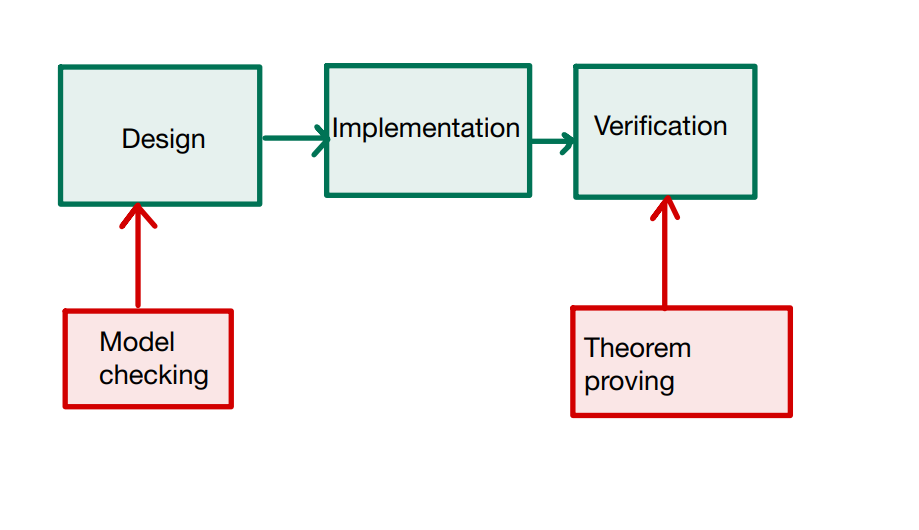
\includegraphics[width=\textwidth]{img/2.png}
\end{frame}

\begin{frame}[fragile]
	\begin{lstlisting}[language=C++]

void main() {
    int i = getValue(); // start
    i++; // middle
    setValue(i); // done
}

	\end{lstlisting}
	
\end{frame}

\begin{frame}
    \begin{center}
        \LARGE{\textbf{How to model this simple program formally as state machine?}}
    \end{center}

\end{frame}

\begin{frame}
    \frametitle{State diagram}
    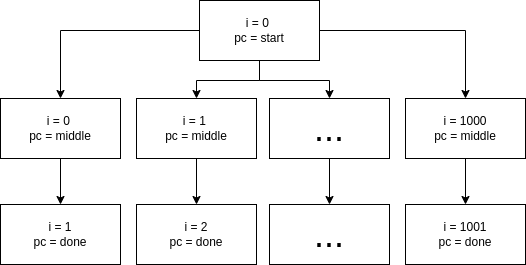
\includegraphics[width=0.9\textwidth, height=0.9\textheight]{img/1.png}
\end{frame}


\begin{frame}[fragile]
	\begin{lstlisting}[language=C++]


void thread2() {
    int i = getValue();
    i++;
    setValue(i);
}

void thread1() {
    int i = getValue();
    i++;
    setValue(i);
}

	\end{lstlisting}
	
\end{frame}

\begin{frame}[fragile]
    \frametitle{Networked program}
	\begin{lstlisting}[language=C++]

void processRequest() {
    Message *msg = receiveMessage();
    if (msg->type == CLIENT_REQUEST) {
        ...
    } else {
        ...
    }
    for (auto node : getNodes()) {
        node->sendMessage(NODE_REQUEST);
    }
}

	\end{lstlisting}
	
\end{frame}

\begin{frame}
    \frametitle{TLA+}
    \begin{itemize}
        \item Essentially we specify state machine and its properties 
        \begin{itemize}
            \item State variables
            \item What are valid initial states 
            \item What are valid next states, given current state 
            \item Properties
        \end{itemize}
        \item TLC is used for model checking 
    \end{itemize}
\end{frame}

\begin{frame}[fragile]
	\begin{lstlisting}[language=C++]

void main() {
    int i = getValue(); // start
    i++; // middle
    setValue(i); // done
}

	\end{lstlisting}
	
\end{frame}

\begin{frame}[fragile]
    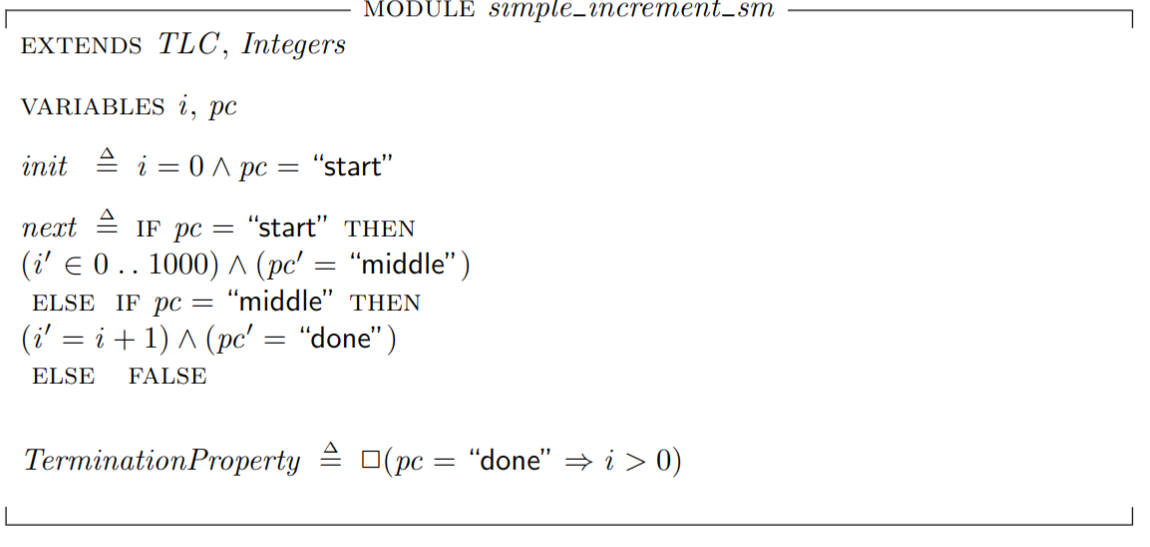
\includegraphics[width=\textwidth]{./sm_increment.png}
\end{frame}

\begin{frame}
    \frametitle{PlusCal}
    \begin{itemize}
        \item A little more programmer-friendly 
        \item We specify processes and TLC will check all behaviours
    \end{itemize}
\end{frame}


\begin{frame}[fragile]
    \frametitle{Real world example - health monitor}
    \begin{itemize}
        \item We have several nodes (lets say nodes are 1, 2 and 3)
        \item Every node can reboot and recover later on 
        \item Every node has one instance of service 
        \item When node is down, its service instance gets transferred to another node which is up to serve additional traffic
        \item When we detect that service instance is stuck, we kill it and restart it 
        \item We state that eventually if service is stuck, this will lead to either it being killed or recovered by itself
    \end{itemize}
\end{frame}

\begin{frame}
    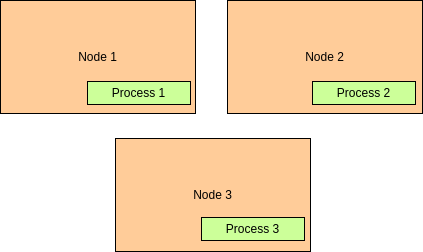
\includegraphics[width=0.9\textwidth, height=0.9\textheight]{img/scenario_1.drawio.png}
\end{frame}



\begin{frame}
    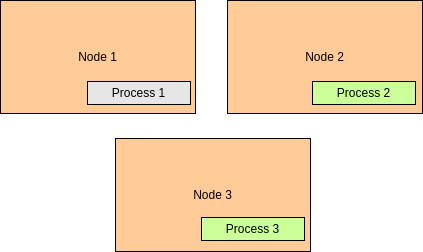
\includegraphics[width=0.9\textwidth, height=0.9\textheight]{img/scenario_2.drawio.png}
\end{frame}


\begin{frame}
    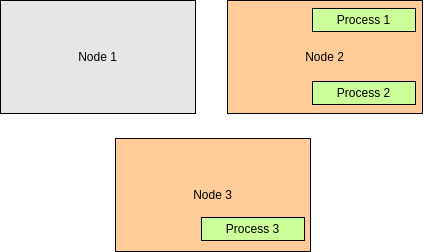
\includegraphics[width=0.9\textwidth, height=0.9\textheight]{img/scenario_3.drawio.png}
\end{frame}


\begin{frame}
    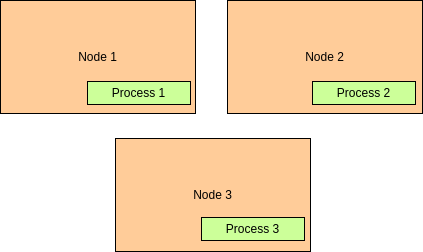
\includegraphics[width=0.9\textwidth, height=0.9\textheight]{img/scenario_4.drawio.png}
\end{frame}


\begin{frame}
    \begin{center}
        \LARGE{\textbf{Demo}}
    \end{center}

\end{frame}

\begin{frame}
    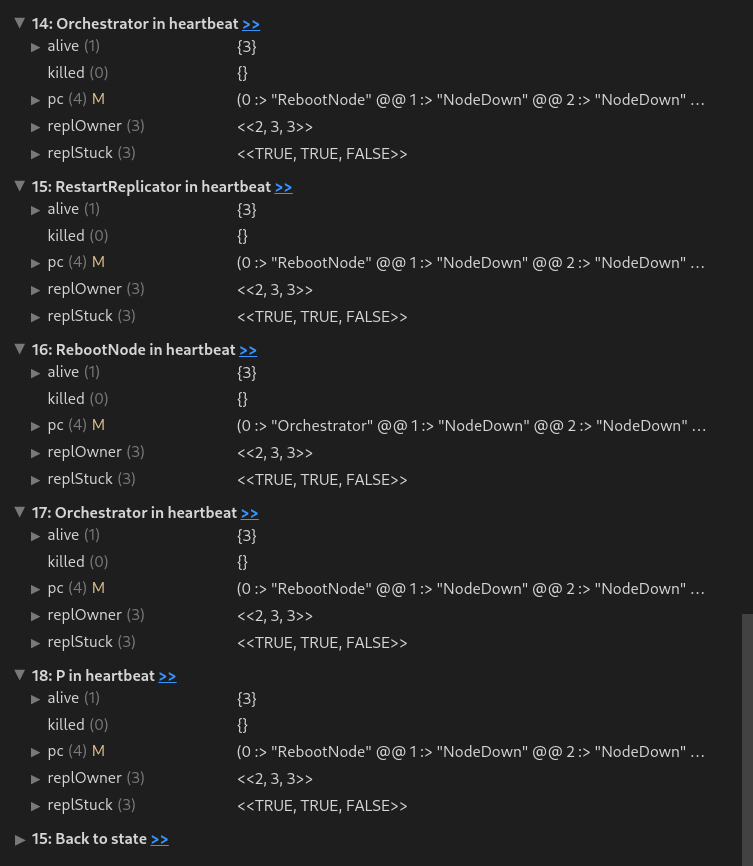
\includegraphics[width=0.9\textwidth, height=0.9\textheight]{examples/img1.png}
\end{frame}


\begin{frame}
    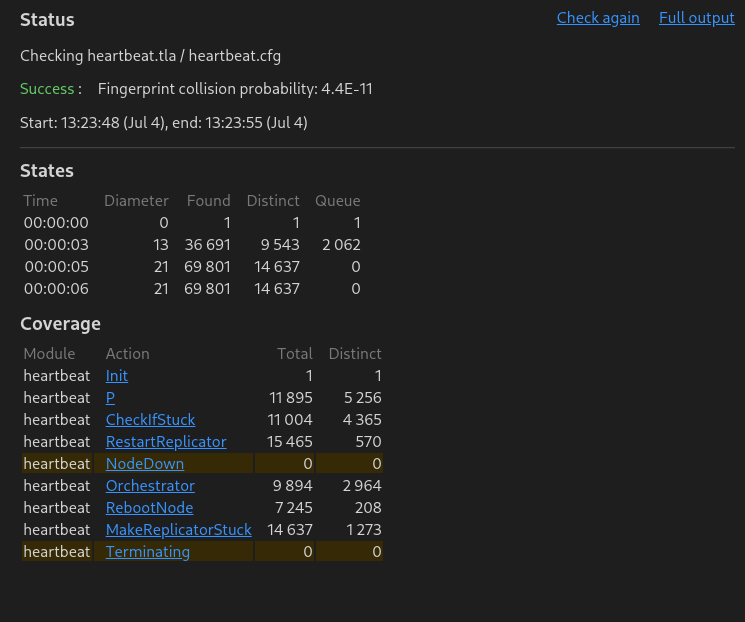
\includegraphics[width=0.9\textwidth, height=0.9\textheight]{examples/img2.png}
\end{frame}


\begin{frame}
    \frametitle{Conclusion}
    \begin{itemize}
        \item Formal specification can help us reason about systems and communicate better in teams
        \item There are tools to help us formally specify systems and to check its validity 
        \item More granular we go, more validation we get
        \item We can specify various kinds of systems and check various kinds of things
        \begin{itemize}
            \item Termination
            \item Security
            \item Correctness for given level of granularity
        \end{itemize}
    \end{itemize}
\end{frame}

\begin{frame}
    \begin{center}
        \LARGE{\textbf{Gossip session}}
    \end{center}

\end{frame}

\end{document}
